 \section{Implementacja komunikacji}
      \subsection{Łączenie z brokerem}
        Podobnie jak w framework'u użytym na poczet przygotowania wsadu do sterownika, tutaj również jest zdefiniowana fenomenalnie prosta w obsłudze abstrakcja. Niemniej jednak w celu utrzymania wysokiej czytelności produkowanego kodu została przygotowana nowa autorska klasa. Dziedziczy ona po klasie zawartej w module QtMqtt. Jej celem jest rozszerzenie klasy bazowej o dodatkową funkcjonalność, która sprawi że inicjalizacja i obsługa połączenia będą jeszcze wygodniejsze. Jako argumenty wywołania należy podać adres i port serwera, a następnie nazwę użytkownika oraz hasło. Cała reszta procesu została zgrabnie ukryta pod warstwą abstrakcji. Omawiany kod przedstawiony został w listingu \ref{code:app_mqtt_connection}.
        
                
       \begin{figure}[ht]
          \centering
          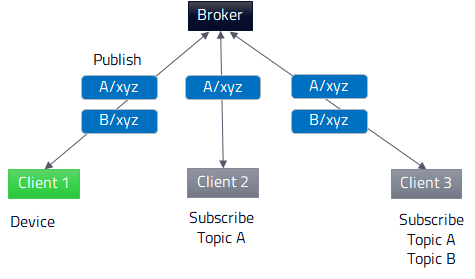
\includegraphics[width=0.8\textwidth]{img/qt_mqtt.png}
          \caption{Schemat działania modułu Qt MQTT \cite{qt_mqtt_fig}}
          \label{fig:qt_mqtt}
        \end{figure}   
        
        \begin{kod}
          \inputminted[firstline=21, lastline=34]{cpp}{app/listings/mqtt.cpp}
          \caption{Nawiązanie połączenia z brokerem}
          \label{code:app_mqtt_connection}
        \end{kod}
        
      \subsection{Obsługa zdarzeń}
        Kolejną analogią znaną z frameworka ESP-IDF jest obsługa zdarzeń przychodzących z modułu MQTT. Wysyła on sygnał połączony z funkcją widoczną w listingu \ref{code:app_mqtt_state} zdający raport o stanie połączenia. Jest on wykorzystywany do aktywowania interfejsu użytkownika, który domyślnie przyjmuje status nieaktywnego. Ponadto jest to wyzwalacz do subskrybowania uprzednio zdefiniowanych tematów.
        \begin{kod}
          \inputminted[firstline=102, lastline=127]{cpp}{app/listings/mainwindow.cpp}
          \caption{Obsługa zdarzeń}
          \label{code:app_mqtt_state}
        %   \vspace{2em}
        \end{kod}
        
        
      \subsection{Subskrybowanie tematów}
        Subskrybowanie tematów jest dość długą funkcją. Wbrew pozorom nie jest ona skomplikowana. Jej zadaniem jest zasubskrybować jedynie cztery temat. Z tego też powodu wszystko jest powielone czterokrotnie. To właśnie wpływa w znaczący sposób na jej objętość. Dla każdego tematu wywoływana jest metoda na obiekcie MQTT, która przyjmuje temat oraz parametr QoS. 
        
        QoS z angielskiego "Quality of Service" określa poziom istotności wiadomości. W tym przypadku użyta została wartość $0$. Oznacza to że nie ma gwarancji otrzymania wiadomość. Taka kolej rzeczy nie wydaje się być z żaden sposób problematyczna ze względu na cykliczność z jaką otrzymywane są ramki. Zgubienie jednej wartości nie musi być istotne w momencie, gdy są one transmitowane z ponadprzeciętnie dużą częstotliwością. W takim systemie pierwszoplanowa jest wydajność i przepustowość. Pozostałe wartości które są możliwe do ustawienia to $1$ i $2$. Pierwsza z nich sprawia że mamy pewność otrzymania wiadomości, natomiast druga gwarantuje jednokrotność tego zdarzenia.
        
        Produktem wywołania tej metody będzie obiekt typu QMqttSubscription, który następnie należy przy pomocy systemu sygnałów i slotów, połączyć z odpowiednią funkcją. Funkcja ta jedynie skleja otrzymaną wartość z uprzednio przygotowanym ciągiem znaków i bezpośrednio wyświetla ją w interfejsie użytkownika. Przykład takiej funkcji dostępny jest w listingu \ref{code:app_mqtt_setValue}. 
        
        Na samym końcu znajduje się jeszcze wywołanie funkcji ustawiającej wartości domyślne dla wyżej wymienionych tematów, tak aby można było je umieścić w interfejsie. Cała ta procedura powtórzona jest cztery razy dla czterech różnych tematów. Odnosi się do niej listing \ref{code:app_mqtt_subscribe}. 

        
        \begin{kod}
          \inputminted[firstline=245, lastline=254]{cpp}{app/listings/mainwindow.cpp}
          \caption{Przetwarzanie odebranych danych}
          \label{code:app_mqtt_setValue}
        \end{kod}
        
      
        \begin{kod}
          \inputminted[firstline=186, lastline=205]{cpp}{app/listings/mainwindow.cpp}
          \caption{Subskrybowanie tematów}
          \label{code:app_mqtt_subscribe}
          \vspace{1em}
        \end{kod}
        
        
      \subsection{Wysyłanie danych}
        Wysyłanie danych polega na odbieraniu wartości prosto z interfejsu i przekazywaniu ich do metody obiektu MQTT. Połączone są więc konkretne sygnały elementów interfejsu z daną lambdą. W roli przykładu, sygnał suwaka ustawiającego wartość zadaną łączymy z lambdą w której wyłuskujemy wartość suwaka. Następnie jest ona zapisywana jako tablica bajtów i publikowana. Dodatkowo jest wyświetlana w postaci liczbowej w interfejsie. Przykład implementacji znajduje się w listingu \ref{code:app_mqtt_send}.
        
        \begin{kod}
          \inputminted[firstline=208, lastline=235]{cpp}{app/listings/mainwindow.cpp}
          \caption{Wysyłanie danych}
          \label{code:app_mqtt_send}
          \vspace{2em}
        \end{kod}       
        